\documentclass{article}

\usepackage{datatool}
\DTLsetseparator{ = }
\DTLloaddb[noheader, keys={mykey,myvalue}]{myvars}{ripplevars.py}
\newcommand{\var}[1]{\DTLfetch{myvars}{mykey}{#1}{myvalue}}

\usepackage{tikz}
\usetikzlibrary{patterns}

\usepackage{listings}

\usepackage[margin=1in]{geometry}

\title{Ripples}
\author{Hunter Damron}
\date{1 March 2019}

\newcommand{\block}[2]{\fill (#1,#2) rectangle (#1+1,#2+1);}
\newcommand{\checker}[1]{
	\foreach \y in {-#1,...,#1} {
		\draw (-#1,\y) -- (#1,\y);
	}
	\foreach \x in {-#1,...,#1} {
		\draw (\x,-#1) -- (\x,#1);
	}
}

\begin{document}
	\maketitle

	\section*{Problem Description}
	In an oddly square world, ripples do not radiate from the source as a ring but rather as a diamond as demonstrated in Figure~\ref{fig:ripple}. Note that when a wave meets the end of the defined world, it wraps around as if the world is toroidal. And, when waves collide, they cancel each other in that time instance (each wave still moves after that time instance in its previous direction). However, if more than two wave points collide, each pair of wave points cancels. This cancellation is only present for a single time step, however, as waves continue to propagate after collisions. Assume the bottom left cell of the world is index $(0,0)$ with right as $+x$ and up as $+y$.

	\begin{figure}[h!]
		\centering
		\caption{Evolution of the waves. The small circle denotes the location of a dropped object at time 0 and filled squares denote wave points. Shaded squares denote collided waves and are labelled only for demonstration.} \label{fig:ripple}
		\begin{tabular}{cc}
		$t=0$ & $t=2$ \\
		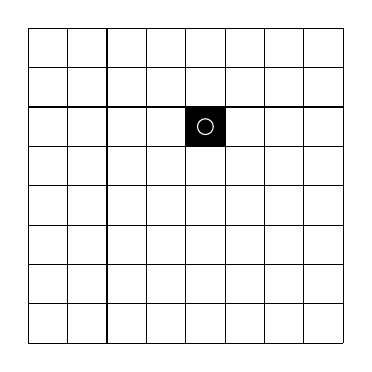
\begin{tikzpicture}[scale=0.5]
			\checker{4};
			\block{0}{1};
			\draw[white] (0.5,1.5) circle (0.2cm);
		\end{tikzpicture}
		&
		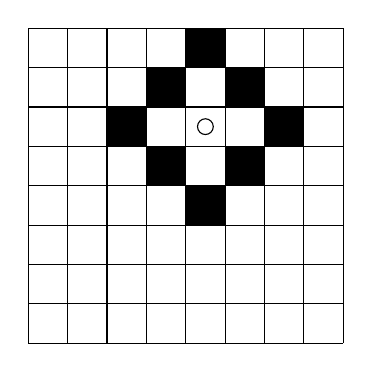
\begin{tikzpicture}[scale=0.5]
			\checker{4};
			\foreach \r in {0,...,2} {
				\block{2-\r}{1+\r};
				\block{2-\r}{1-\r};
				\block{-2+\r}{1+\r};
				\block{-2+\r}{1-\r};
			}
			\draw (0.5,1.5) circle (0.2cm);
		\end{tikzpicture}
		\\[1em]
		$t=3$ & $t=4$ \\
		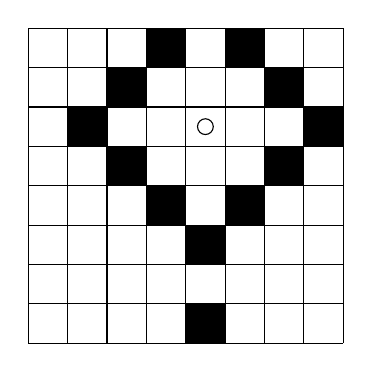
\begin{tikzpicture}[scale=0.5]
			\checker{4};
			\block{0}{-4};
			\foreach \r in {0,...,3} {
				\block{3-\r}{1-\r};
				\block{-3+\r}{1-\r};
			}
			\foreach \r in {0,...,2} {
				\block{3-\r}{1+\r};
				\block{-3+\r}{1+\r};
			}
			\draw (0.5,1.5) circle (0.2cm);
		\end{tikzpicture}
		&
		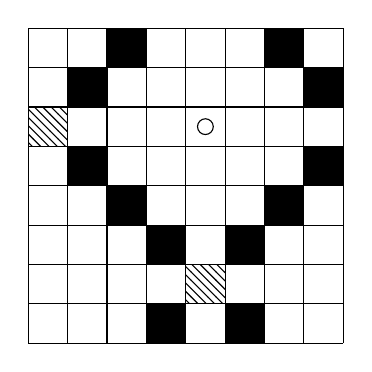
\begin{tikzpicture}[scale=0.5]
			\checker{4};
			\block{-1}{-4};
			\block{1}{-4};
			\foreach \r in {1,...,3} {
				\block{4-\r}{1-\r};
				\block{-4+\r}{1-\r};
			}
			\foreach \r in {1,...,2} {
				\block{4-\r}{1+\r};
				\block{-4+\r}{1+\r};
			}
			\draw (0.5,1.5) circle (0.2cm);
			\draw[pattern=north west lines] (0,-3) rectangle (1,-2);
			\draw[pattern=north west lines] (-4,2) rectangle (-3,1);
		\end{tikzpicture}
		\end{tabular}
	\end{figure}

	\section*{Inputs}
	The input is specified as follows:
	\begin{enumerate}
		\item The first line specifies three space-separated integers: width ($w$), height ($h$), and the number of dropped objects ($n$)
		\item The next $n$ lines each have three space separated integers: time ($t_i$), $x$-position ($x_i$), and $y$-position ($y_i$) of drop number $i$
		\item The final line specifies the time of interest $t_f$
	\end{enumerate}

	\noindent
	The following constraints are placed on the variables:
	\begin{itemize}
		\item $0 < w \leq \var{maxw}$
		\item $0 < h \leq \var{maxh}$
		\item $0 < n \leq \var{maxn}$

		\item $0 \leq t_i < \var{maxt}$
		\item $0 \leq x_i < w$
		\item $0 \leq y_i < h$

		\item $\max_i(t_i) < t_f$
	\end{itemize}

	\section*{Desired Output}
	Rather than printing the whole world at time $t_f$ (because that could be quite large!), count the number of wave points present (and not canceled) at time $t_f$. In the example above, the output would be 12.

	\section*{Samples}
	The sample from above is shown in Sample 0. Sample 1 shows a variation of Sample 0 with multiple drops, including one which occurs as $t_f$. Sample 2 shows a harder scenario like the ones which will be tested against. Each sample shows the verbatim input on the left side and the corresponding output on the right.
	\newcommand{\sample}[1]{
		\begin{tabular}{|c|c|}
			\hline
			\lstinputlisting{input/input#1.txt} & \lstinputlisting{output/output#1.txt} \\
			\hline
		\end{tabular}
	}
	\begin{table}[h!]
		\centering
		\setlength{\tabcolsep}{1em}
		\begin{tabular}{c}
			Sample 0 \\
			\sample{0} \\\\
			Sample 1 \\
			\sample{1} \\\\
			Sample 2 \\
			\sample{2}
		\end{tabular}
	\end{table}
\end{document}
